\documentclass[a4paper, 12pt]{article}

% Packages
\usepackage[portuguese,english]{babel}
\usepackage[utf8]{inputenc}
\usepackage[T1]{fontenc}
\usepackage{geometry}
  \geometry{margin=1in}
\usepackage{amsmath}
\usepackage{graphicx}
\usepackage{hyperref}

\title{\bf Comparação de Algoritmos de Ordenação}
\author{%
    Kaíque M. Lima \\
    Universidade Tecnológica Federal do Paraná (UTFPR) \\
    Santa Helena, PR -- Brasil\\[1ex]
    Pesquisa e Ordenação -- Prof. Glória Patrícia Lopez Sepulveda\\
    {\small \texttt{kaiquelima@alunos.utfpr.edu.br}}
}
\date{}  % sem data

\begin{document}
\maketitle

\begin{abstract}
    \textit{
        This report presents an empirical comparison of eight sorting algorithms implemented in C++ (Bubble, Insertion, Shell, Selection, Merge, Quick, Radix, and Heap), evaluated under three input scenarios (sorted, reverse‐sorted, and random) on up to 1.35 million elements on a single machine. The results make it clear that the quadratic algorithms (Bubble, Insertion, and Selection) are infeasible for large data volumes, while Random‐Pivot Quick Sort and Heap Sort offer the best balance of average performance and robustness. Shell Sort performs surprisingly well in adverse cases, but the overhead of Radix Sort limits its theoretical advantage. We conclude that algorithm choice must consider not only asymptotic complexity but also memory‐access patterns, space usage, and data‐specific characteristics—there is no one-size-fits-all solution.
    }
\end{abstract}

\selectlanguage{portuguese}
\begin{abstract}
    \textit{
        Este relatório apresenta uma comparação empírica de oito algoritmos de ordenação implementados em C++ (Bubble, Insertion, Shell, Selection, Merge, Quick, Radix e Heap), avaliados em três cenários de entrada (ordenados, invertidos e aleatórios) para até 1,35 milhão de elementos em uma máquina. Os resultados deixam claro que os algoritmos quadráticos (Bubble, Insertion e Selection) são inviáveis para grandes volumes de dados, enquanto Quick Sort com pivô aleatório e Heap Sort oferecem o melhor equilíbrio entre desempenho médio e robustez. Shell Sort surpreende em casos adversos, mas o overhead de Radix Sort limita sua vantagem teórica. Conclui-se que a escolha do método deve considerar não só a complexidade assintótica, mas também padrões de acesso à memória, uso de espaço e características específicas dos dados — não há “tamanho único” que sirva para todas as situações.
        }
\end{abstract}

% Introdução
\section{Introdução}

    Esse relatório apresenta uma análise comparativa de 8 algoritmos de ordenação: Bubble Sort, Insertion Sort, Shell Sort, Selection Sort, Merge Sort, Quick Sort, Radix Sort e Heap Sort. A comparação é feita com base em gráficos que mostram o tempo de execução em função do tamanho do arquivo a ser ordenado. Os testes foram realizados na linguagem C++, em uma máquina com as seguintes especificações: I3-10100f, RTX 2060 e 16GB de RAM.
    O objetivo é entender o desempenho de cada algoritmo em diferentes cenários e tamanhos de entrada, além de discutir suas características, vantagens e desvantagens. A análise inclui tanto algoritmos de ordenação baseados em comparação quanto não comparativos, permitindo uma visão abrangente das técnicas de ordenação disponíveis.

% Descrição da atividade
\section{Descrição da atividade}
    \subsection{Algoritmos e seus tempos de execução}
        \subsubsection{Bubble Sort}
            Bubble Sort faz sucessivas passagens comparando e trocando elementos adjacentes fora de ordem até não haver mais trocas. Seu tempo é quadrático (O(n²)) na maioria dos casos e linear só quando a lista já está ordenada. Por ser estável e simples, serve apenas para ensino ou dados minúsculos; em qualquer cenário real, seu desempenho é ineficaz. O algotitmo em questão usado no projeto foi otimizado, conferindo se nenhuma troca foi feita na última passagem. Se não houver trocas, o algoritmo termina, evitando passagens desnecessárias.

            \begin{figure}[ht]
                \centering
                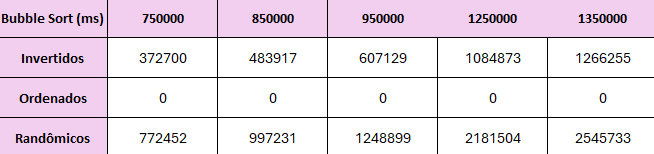
\includegraphics[width=0.8\textwidth]{images/bubble.png}
            \end{figure}

        \subsubsection{Insertion Sort}
            Insertion Sort constrói progressivamente a parte ordenada inserindo cada novo elemento em seu lugar correto, deslocando os maiores. Em média é O(n²), mas cai a O(n) se o array estiver quase ordenado. Como exige pouquíssima sobrecarga, é adotado em implementações híbridas (por exemplo, em Quick Sort recursivo quando as partições ficam pequenas) ou em listas pequenas.

            \begin{figure}[ht]
                \centering
                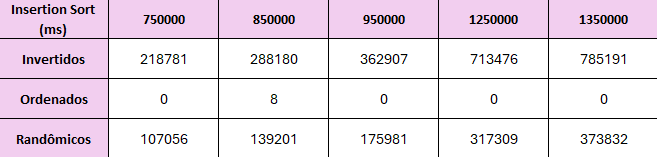
\includegraphics[width=0.8\textwidth]{images/insertion.png}
            \end{figure}

        \subsubsection{Shell Sort}
            Shell Sort aprimora o Insertion Sort usando uma sequência de “gaps” para comparar e trocar elementos distantes, reduzindo inversões antes da fase final com gap = 1. Seu comportamento depende da escolha de gaps e fica entre O(n log² n) e O(n(1.5)), sem ser estável. É razoável para tamanhos médios quando se busca algo simples e in-place, mas algoritmos mais modernos usualmente o superam.

            \begin{figure}[ht]
                \centering
                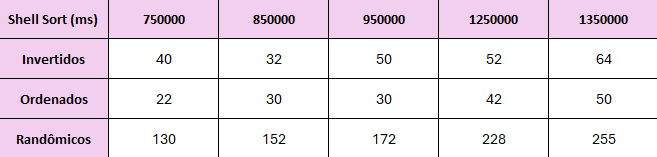
\includegraphics[width=0.8\textwidth]{images/shell.png}
            \end{figure}

        \subsubsection{Selection Sort}
            Selection Sort encontra repetidamente o menor (ou maior) elemento na porção não ordenada e o coloca na posição correta por troca. Independentemente da entrada, sempre faz O(n²) comparações e poucas trocas (O(n)). Por não ser estável e ter custo quadrático, só vale a pena em coleções diminutas ou em situações em que escrita em memória seja extremamente custosa. É ineficiente mesmo em arquivos odenados.

            \begin{figure}[ht]
                \centering
                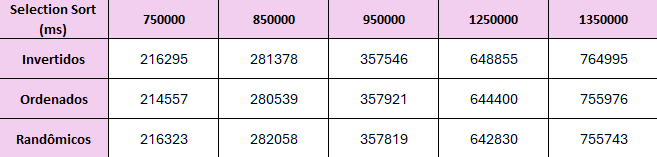
\includegraphics[width=0.8\textwidth]{images/selection.png}
            \end{figure}

        \subsubsection{Merge Sort}
            Merge Sort divide recursivamente o vetor ao meio, ordena cada metade e mescla os resultados. Seu tempo de execução é sempre O(n log n) e requer O(n) de espaço extra para as fusões. Por manter estabilidade e oferecer desempenho previsível, é indicado para conjuntos grandes ou para ordenação externa, mas o consumo de memória o torna menos atrativo quando há restrição de espaço e por ser recursivo pode levar a stack overflow.

            \begin{figure}[h]
                \centering
                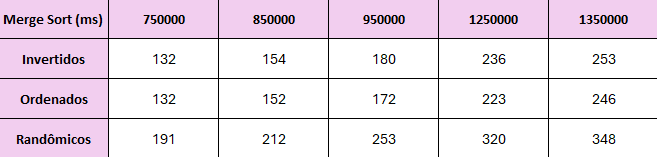
\includegraphics[width=0.8\textwidth]{images/merge.png}
            \end{figure}

        \subsubsection{Quick Sort}
            Quick Sort escolhe um pivô, particiona o array em elementos menores e maiores que ele e aplica recursão nas partições. Em média é O(n log n) com espaço de pilha O(log n), mas pode degradar para O(n²) em casos patológicos de pivô mal escolhido. É o mais rápido na prática para a maioria dos usos gerais, desde que se evitem entradas adversas ou se adote estratégias de escolha do pivô mais robustas. Nesse caso, o algoritmo usado foi o de escolha aleatória do pivô, que evita os casos degenerados. O algoritmo também foi otimizado para evitar recursão em partições pequenas.

            \begin{figure}[ht]
                \centering
                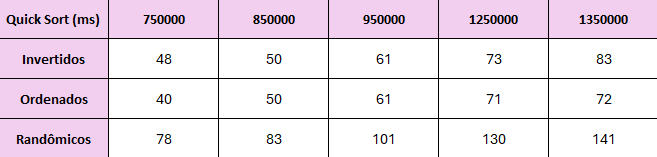
\includegraphics[width=0.8\textwidth]{images/quick.png}
            \end{figure}

        \subsubsection{Radix Sort (LSD)}
            Radix Sort é um algoritmo não comparativo que ordena inteiros processando cada dígito, do menos ao mais significativo, agrupando-os em “baldes” a cada passagem. Ele executa em tempo linear relativo ao número de dígitos (O(d·(n+k))) e consome espaço extra proporcional a n + k, tornando-o útil apenas para grandes conjuntos de inteiros de tamanho fixo – para dados menores o overhead praticamente anula qualquer vantagem, mas não tão eficaz quando os números são muito grandes.

            \begin{figure}[ht]
                \centering
                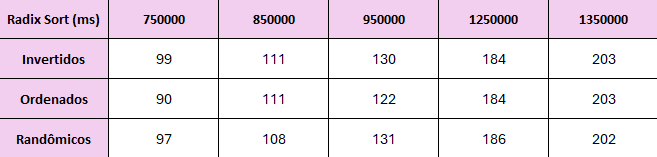
\includegraphics[width=0.8\textwidth]{images/radix.png}
            \end{figure}

        \subsubsection{Heap Sort}
            Heap Sort constrói um heap binário a partir da lista e, a cada extração do maior (ou menor) elemento, reconstrói o heap até esvaziá-lo. Tem custo garantido de O(n log n) em todos os casos e roda in-place com O(1) de espaço adicional. Apesar de previsível, costuma ser mais lento que Quick Sort na prática por ter padrões de acesso menos amigáveis ao cache e não preservar estabilidade.

            \begin{figure}[ht]
                \centering
                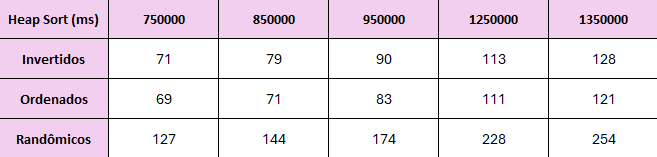
\includegraphics[width=0.8\textwidth]{images/heap.png}
            \end{figure}
    \subsection{Análise por Tipo de Entrada}
        Nesta seção, analisamos o comportamento dos algoritmos em três cenários distintos: dados inversamente ordenados, dados já ordenados e dados em ordem aleatória.

        \subsubsection{Dados Inversamente Ordenados}
            Quando os números estão em ordem decrescente, a entrada representa o pior caso para vários algoritmos. Observamos que:

            \begin{itemize}
                \item O Bubble Sort e Insertion Sort tiveram desempenho extremamente ruim, com tempos de execução próximos a 2.54 milhões de milissegundos para entradas de 1.35 milhão de elementos, confirmando sua complexidade O(n²) no pior caso.
                \item Selection Sort também apresentou comportamento quadrático com aproximadamente 765.000 ms para o mesmo tamanho de entrada.
                \item Quick Sort surpreendentemente manteve bom desempenho (83 ms para 1.35M elementos) graças à implementação com pivô randômico, evitando o caso degenerado.
                \item Heap Sort foi consistentemente rápido (128 ms para 1.35M elementos), demonstrando que sua complexidade O(n log n) se mantém mesmo em cenários adversos.
                \item Shell Sort teve desempenho notável (64 ms para 1.35M elementos), superando até mesmo algoritmos teoricamente mais eficientes.
            \end{itemize}

            \begin{figure}[ht]
                \centering
                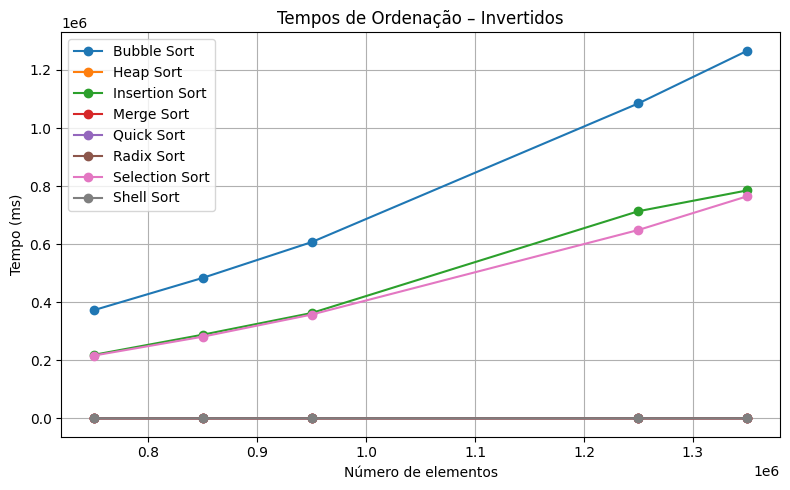
\includegraphics[width=0.8\textwidth]{images/invertidos.png}
            \end{figure}

        \subsubsection{Dados Ordenados}
            Quando os números já estão ordenados, observamos comportamentos interessantes:

            \begin{itemize}
                \item Bubble Sort teve desempenho ótimo, com tempo praticamente zero, pois identifica a ordenação na primeira passagem.
                \item Insertion Sort também se mostrou extremamente eficiente com tempo quase zero, confirmando sua complexidade O(n) para dados já ordenados.
                \item Heap Sort, Merge Sort e Quick Sort mantiveram seus tempos O(n log n) independentemente da ordenação prévia (respectivamente 121 ms, 246 ms e 72 ms para 1.35M elementos).
                \item Radix Sort não se beneficiou da ordenação prévia (203 ms para 1.35M elementos), demonstrando que seu desempenho depende mais do número de dígitos que da ordem inicial.
                \item Shell Sort mostrou-se muito eficiente (50 ms para 1.35M elementos), adaptando-se bem a dados já ordenados.
            \end{itemize}

            \begin{figure}[ht]
                \centering
                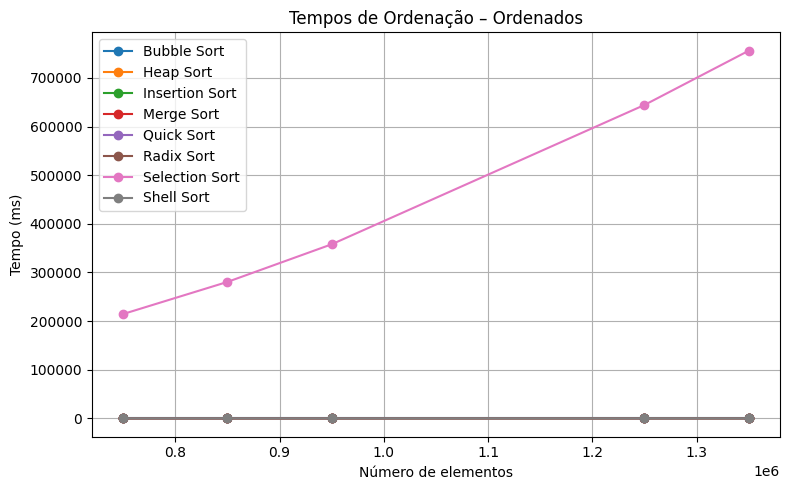
\includegraphics[width=0.8\textwidth]{images/ordenados.png}
            \end{figure}

        \subsubsection{Dados Aleatórios}
            Com entradas aleatórias, que representam o caso médio, observamos:

            \begin{itemize}
                \item Bubble Sort teve desempenho catastrófico (2.54 milhões ms para 1.35M elementos), mostrando por que não deve ser usado em aplicações reais.
                \item Quick Sort confirmou sua reputação como algoritmo mais eficiente na prática para casos médios (141 ms para 1.35M elementos).
                \item Heap Sort e Shell Sort apresentaram desempenho similar (254 ms e 255 ms para 1.35M elementos), mostrando que o Shell Sort pode competir com algoritmos mais sofisticados em determinados cenários.
                \item Radix Sort teve boa performance (202 ms para 1.35M elementos), mas sem superar significativamente o Quick Sort, apesar de sua complexidade teórica linear.
                \item Merge Sort foi mais lento que o esperado (348 ms para 1.35M elementos), possivelmente devido ao overhead de alocação de memória.
            \end{itemize}

            \begin{figure}[ht]
                \centering
                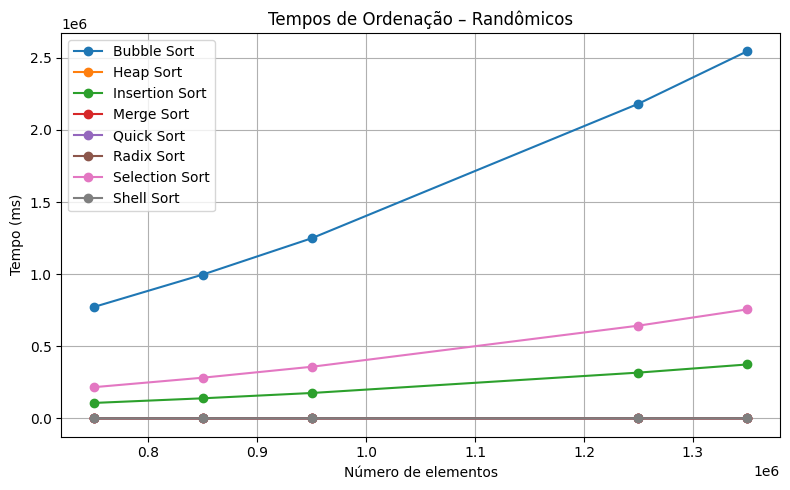
\includegraphics[width=0.8\textwidth]{images/randomicos.png}
            \end{figure}

    \subsection{Comparação Geral}
        Analisando o desempenho geral dos algoritmos nos diferentes cenários, podemos concluir que:


        \begin{itemize}
            \item Quick Sort mostrou o melhor equilíbrio entre eficiência e consistência, sendo o algoritmo mais rápido na maioria dos cenários quando implementado com escolha aleatória de pivô.
            \item Shell Sort surpreendeu positivamente, com desempenho comparável a algoritmos teoricamente mais eficientes, especialmente em dados inversamente ordenados.
            \item Heap Sort demonstrou sua estabilidade de desempenho, mantendo tempos similares independentemente do tipo de entrada.
            \item Algoritmos quadráticos (Bubble, Insertion e Selection Sort) são inviáveis para grandes volumes de dados, exceto em casos específicos como o Insertion Sort para dados quase ordenados.
                \item Radix Sort, apesar de sua complexidade linear, não superou consistentemente os melhores algoritmos de comparação, provavelmente devido ao overhead das passagens por dígito.
            \end{itemize}

            \begin{figure}[ht]
                \centering
                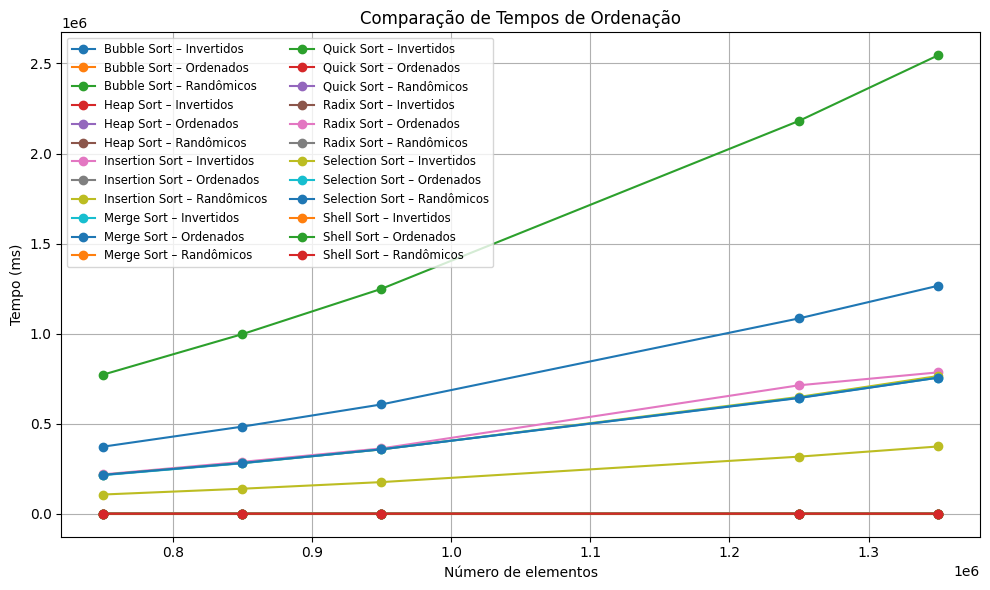
\includegraphics[width=0.9\textwidth]{images/tudoqueda.png}
            \end{figure}



            Esta análise confirma que a escolha do algoritmo de ordenação deve considerar não apenas a complexidade teórica, mas também características da entrada, requisitos de estabilidade, uso de memória e padrões de acesso que podem afetar o desempenho em sistemas reais.

    % Conclusão
    \section{Conclusão}
    Este estudo comparativo de oito algoritmos de ordenação revelou insights importantes sobre seus comportamentos e eficiência em diferentes cenários. Os resultados obtidos demonstram claramente que não existe um único algoritmo "melhor" para todas as situações, confirmando a importância de conhecer as características específicas de cada método.

    O Quick Sort com pivô aleatório destacou-se como o algoritmo mais versátil e eficiente na maioria dos cenários, enquanto o Shell Sort surpreendeu com desempenho competitivo apesar de sua menor complexidade teórica. O Heap Sort demonstrou notável consistência independentemente da distribuição dos dados, o que o torna uma escolha confiável em contextos onde o pior caso deve ser evitado. Em contrapartida, os algoritmos quadráticos (Bubble, Insertion e Selection Sort) confirmaram sua inviabilidade para grandes volumes de dados, exceto em situações específicas como dados já ordenados para o Insertion Sort.

    O Radix Sort, apesar de sua complexidade linear teórica, não conseguiu superar consistentemente os melhores algoritmos baseados em comparação, indicando que os fatores constantes e o overhead de processamento por dígito podem ter impacto significativo no desempenho real.

    Para aplicações práticas, este estudo sugere que:
    \begin{itemize}
        \item Para uso geral com grandes volumes de dados, o Quick Sort com pivô aleatório oferece o melhor equilíbrio entre eficiência média e robustez;
        \item Em situações onde o desempenho do pior caso é crítico, Heap Sort ou Merge Sort são alternativas mais seguras;
        \item Para conjuntos pequenos ou parcialmente ordenados, Insertion Sort pode ser surpreendentemente eficaz;
        \item Shell Sort merece mais atenção em aplicações práticas do que sua popularidade atual sugere.
    \end{itemize}

    Finalmente, esta análise reforça a importância de considerar fatores além da complexidade assintótica teórica na escolha de algoritmos de ordenação, incluindo padrões de acesso à memória, localidade de cache, estabilidade e características específicas dos dados de entrada. Em sistemas reais, o conhecimento aprofundado dessas características permite selecionar o algoritmo mais adequado para cada contexto específico, otimizando o desempenho e a eficiência dos sistemas computacionais.

\end{document}
